\documentclass{article}

% if you need to pass options to natbib, use, e.g.:
\PassOptionsToPackage{numbers, compress}{natbib}
% before loading nips_2017
%
% to avoid loading the natbib package, add option nonatbib:
% \usepackage[nonatbib]{nips_2017}

%\usepackage{nips_2017}

% to compile a camera-ready version, add the [final] option, e.g.:
\usepackage[final]{nips_2017}

\usepackage[utf8]{inputenc} % allow utf-8 input
\usepackage[T1]{fontenc}    % use 8-bit T1 fonts
\usepackage{hyperref}       % hyperlinks
\usepackage{url}            % simple URL typesetting
\usepackage{booktabs}       % professional-quality tables
\usepackage{amsfonts}       % blackboard math symbols
\usepackage{nicefrac}       % compact symbols for 1/2, etc.
\usepackage{microtype}      % microtypography
\usepackage{algorithm}
\usepackage[noend]{algpseudocode}
\usepackage{shortcuts}
\usepackage{bm}
\usepackage[dvipsnames]{color}
\usepackage{amsmath,amsthm,amssymb,parskip,setspace,tabularx, wrapfig,float,enumerate} 
\usepackage{tikz, setspace, subfig, grffile}
\usepackage{subfig}
\usetikzlibrary{bayesnet}

\title{Mapping Gaussian Process Priors
\\ to Bayesian Neural Networks}

% The \author macro works with any number of authors. There are two
% commands used to separate the names and addresses of multiple
% authors: \And and \AND.
%
% Using \And between authors leaves it to LaTeX to determine where to
% break the lines. Using \AND forces a line break at that point. So,
% if LaTeX puts 3 of 4 authors names on the first line, and the last
% on the second line, try using \AND instead of \And before the third
% author name.

\author{
  Daniel Flam-Shepherd \\
  University of Toronto \\
  %\texttt{ @cs.cranberry-lemon.edu} \\
  \And
  James Requeima  \\
  University of Cambridge \\
  % \texttt{email} \\
  \AND
  David Duvenaud \\
  University of Toronto \\
  %% Address \\
  %% \texttt{email} \\
}

\begin{document}
% \nipsfinalcopy is no longer used

\maketitle

\section{Introduction and Motivation}
What defines a reasonable prior to use when forming and training Bayesian models 
and Bayesian neural networks? In a recent work, (Ghosh et al 2016) 
apply a horseshoe prior over preactivations of a Bayesian neural network to 
effectively turns off weights that do not help explain the data. That model and 
many Bayesian models view priors solely in parameter space, in this work we move 
forward with viewing priors in function space as well. 

It is difficult to incorporate meaningful prior information about functions to be 
modelled by BNNs since priors are generally specified over the network parameters. 
Often, normal distributions are placed over the weights for convenience and 
are interpreted as a bias toward less complex functions via smaller weights. 
Gaussian processes, on the other hand, have a elegant mechanism for incorporating 
prior beliefs about the underlying function - specifying the mean and covariance functions.
However, Gaussian Process have scalability limitations making Bayesian neural networks 
a more practical model in large data settings. 
In our work, we present an approach to specify a more principled prior for 
Bayesian Neural Networks that can leverage the well studied kernel design techniques from Gaussian process regression.


We consider matching the prior of a Bayesian neural network $\pbnn (\bm f |\bm \phi )$
to the prior of a Gaussian process $\pgp (\bm f | \bm \theta ) $ 
 by minimizing their KL divergence over 
some data distribution of interest $\X \sim p(\X)$. 
We minimize the KL divergence with respect to the initial variational parameters $\bm \phi$ 
of the proposal distribution $q(\B w |\bm \phi)$. 
These variational parameters 
$\bm \phi^* = \{ \bm \mu _{\bm \phi}^* , \log \bm \sigma _{\bm \phi} ^* \} $ 
yield a prior on the BNN weights 
$p(\B w) = \N (\B w |\bm \mu _{\bm \phi}^* , \bm \sigma _{\bm \phi} ^* )\equiv q(\B w | \bm \phi ^*)$. 
Then, variational inference allows us to perform approximate inference in our BNN using this more 
principled prior. In both stochastic optimization steps, we use the reparameterization trick (Kingma; Rezende 2014) 
to sample from the weights $\B w$ and draw functions from our BNN. 
We describe the implementation of both steps in the next section. 




\begin{figure}[h]\centering
\subfloat[BNN ]{\centering
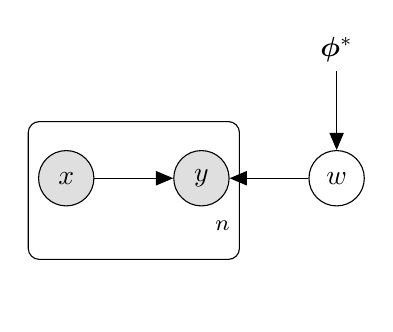
\begin{tikzpicture}[-latex, auto, l/.style={draw,thick,dashed}]
  \node[obs]                               (x) {$\B  x $};
  \node[below=of x]                               (s) {};
  \node[obs, right=of x]                   (y) {$\B  y $};
  \node[latent,right= of y]            (w) {$\B w$};
  \node[above= of w]                    (t) {$\bm \phi ^*$};
  

  % Connect the nodes
  \edge{x}{y};
  \edge{t}{w};
  \edge{w}{y};
  %\path[l] (x) edge [ bend left =40]node[left] {} (f);
        
  % Plates
  \plate[minimum size=1.75cm] {} {(x)(y)} {$n$} ;
\end{tikzpicture}
}
\hspace*{2.5cm}
\subfloat[GP ]{\centering
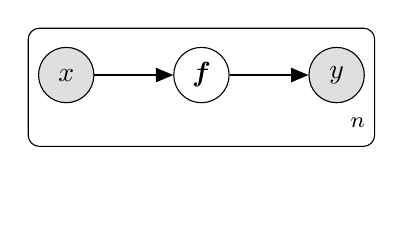
\begin{tikzpicture}[-latex, auto, l/.style={draw,thick,dashed}]
  \node[obs]                               (x) {$\B  x $};
  \node[below=of x]                               (s) {};
  \node[latent, right=of x]                (f) {$\bm f$};
  \node[obs, right=of f]                   (y) {$\B  y $};


  % Connect the nodes
  \edge{x}{f};
  \edge{f}{y};
   \plate[minimum size=1.5cm] {} {(x)(y)} {$n$} ;
 \end{tikzpicture}
}
\caption{ (a) and (b) display the graphical models of a BNN and GP.
} \label{fig:1}
\end{figure}


\newpage
\section{Model Description and Implementation}
\begin{algorithm}
\caption{Optimization of the prior of the Bayesian neural net}
\begin{algorithmic}[1]
\State \textbf{Initialize} $\bm \phi =\{ \bm \mu _{\bm \phi} , \log \bm \sigma _{\bm \phi}  \}$
\While{ $\bm \phi$ not converged}
    \State $ \bm \epsilon ^{(s)} \sim p(\bm \epsilon) = \N (\B 0, \I) $
    \Comment{sample prior noise}
    \State $\B w ^{(s)} \gets g(\bm \phi, \bm \epsilon) = \bm \mu _{\bm \phi} + \bm \sigma _{\bm \phi}\bm \epsilon ^{(s)}$
    \Comment{sample $S$ weights $\B w \sim q(\B w | \phi) $}
    \State $\X \gets ( \B x_1, \dots , \B x_n) \sim p(\B x_1, \dots , \B x_n )$ 
    \Comment{sample data} 
    \State $\bm f ^{(s)} \gets   f_{\tiny\text{NN}}(\B X , \B w^{(s)} )$ 
    \Comment{sample $S$ functions $\bm f \sim \pbnn (\bm f |  \bm \phi )$}
    \State   $\nabla _{\bm \phi} \elbo _{\tiny \X} (\bm \phi )\gets -\frac{1}{S} \sum_s \E_{p(\X)} [\nabla _{\bm \phi}\log \pgp (\bm f ^{(s)}(\B x)| \bm \theta ) ]$
    \Comment{compute gradients of the objective}
    \State $\bm \phi \gets \text{adam}(\bm\phi ,\nabla _{\bm \phi} \elbo _{\tiny \X} (\bm \phi ) )$
    \Comment{update the parameters}
\EndWhile
\State \textbf{Return} $\bm \phi^*$
\end{algorithmic}
\end{algorithm}


\subsection{Step 1. Learn the prior parameters}
In this section we describe the procedure used to minimize the KL divergence of  
the BNN prior distribution over functions $\pbnn (\bm f |  \bm \phi ) $ and
the GP prior distribution over functions  $\pgp (\bm f | \bm \theta )$ 
where $\bm \theta$ are hyperparameters of the kernel $\B K$. 
\begin{align}
    \mathcal K_\X (\bm \phi)&= 
    \kl [\pbnn (\bm f |  \bm \phi ) \mid   \pgp (\bm f | \bm \theta )] 
    = \int\pbnn (\bm f |  \bm \phi ) \log \BB{\frac{\pbnn (\bm f |  \bm \phi ) }{   \pgp (\bm f | \bm \theta )}} d\bm f  \\
    &= -\entropy [\pbnn (\bm f |  \bm \phi ) ] 
       - \E_{\pbnn (\bm f |  \bm \phi ) } [\log \pgp (\bm f | \bm \theta ) ] 
    \propto -\frac{1}{S} \sum_{s=1}^S \log \pgp (\bm f ^{(s)}| \bm \theta ) 
\end{align}

Where we have used a Monte Carlo estimate of 
$ \E_{\pbnn (\bm f |  \bm \phi ) } [\log \pgp (\bm f | \bm \theta ) ]$, 
using S samples $ \bm f ^{(s)} \sim  \pbnn (\bm f |  \bm \phi )$.
We also assume that the entropy term $\entropy [\pbnn (\bm f |  \bm \phi ) ]$ 
is not a function of the variational parameters $\bm \phi$.
We define our first stochastic optimization objective by approximating the KL divergence between these infinite dimensional distributions by taking expectations over where $p(\X)$ allows us to prioritize 
where in the input space we are want $\pbnn (\bm f |  \bm \phi ) \sim \pgp (\bm f | \bm \theta ) $
\begin{align}
     \elbo _\X (\bm \phi)
     &\equiv \E _{\X \sim p(\X)} [\mathcal K_\X (\bm \phi) ]
     \propto - \frac{1}{S} \sum_{s=1}^S  \E_{p(\B X)} [\log \pgp (\bm f ^{(s)}(\B x)| \bm \theta )] 
\end{align}


We optimize (3) until convergence $ \bm \phi ^* =  \amin{\bm \phi}  \elbo _\X (\bm \phi ) $.
This is described in detail in Algorithm 1. 

\subsection{Step 2. Optimize the ELBO}

Next, we use $\bm \phi^*$ found from step 1 to form a prior on the weights  
$p(\B w) =\N ( \B w |  \bm \mu _{\bm \phi} ^*,  \bm \sigma _{\bm \phi}^*)\equiv q(\B w | \bm \phi^*)$. 
Thereafter we learn the parameters 
$\bm \varphi =\{ \bm \mu_{\tiny\bm \varphi} , \log \bm \sigma _{\tiny \varphi} \} $
of the variational approximation 
$q(\B w | \bm \varphi) = \N (\B w |\bm \mu_{\tiny\bm \varphi} , \bm \sigma _{\tiny \varphi} )$ 
to the true posterior on the weights $p(\B w |\D )$. To do this we optimize the evidence lower bound (ELBO) $\elbo (\bm \varphi )$ with our optimized prior $p(\B w ) = q (\B w | \bm \bphi^*   ) $ 
\begin{align}
    \elbo _\D (\bm \varphi ) 
    &=  \E _{q (\B w | \bm \varphi)} \BB{ \log p (\D | \B w ) }  + 
        \kl [q (\B w | \bm \varphi) || q (\B w | \bm \bphi^*  ) ] \\ 
    &=  -\entropy [ q (\B w | \bm \varphi)] + 
        \E _{q (\B w | \bm \varphi)} \BB{ \log p (\D | \B w )  } - 
        \E _{q (\B w | \bm \varphi)} \BB{ \log q (\B w | \bm \bphi^* ) } \\
    &\approx -\log |\bm \sigma _{\tiny \varphi} | + 
         \frac{1}{L}\sum _{\ell=1} ^L \BB{ \log p (\D | \B w ^{(\ell)} )  - \log q (\B w^{(\ell)}  | \bm \bphi^*  ) } \ \text{ where } \B w ^{(\ell)} \sim  q (\B w | \bm \varphi) 
\end{align}

We do this by sampling from a deterministic function of the variational parameters $\bm \varphi$ and noise variables 
$\bm \epsilon \sim p(\bm \epsilon) = \N (\B 0 , \I)$ such that 
$\B w ^{(\ell)} = g(\bm \varphi, \bm \epsilon)= \bm \mu _{\bm \varphi} + \bm \sigma _{\bm \varphi}\bm \epsilon ^{(\ell)} $.
Thus we can obtain unbiased stochastic gradients of the ELBO
with respect to the variational parameters. We use adam (Kingma and Ba 2015) to optimize (6) and (3).



\newpage 
\section{Experiments and results}
We test our model on 3 different toy problems and compare to a Bayesian neural network using a standard
normal prior distribution on the weights trained with bayes by backprop (Blundell et al 2015). 
For the Gaussian process prior, we have $ \pgp (\bm f | \bm \theta ) \sim \N (\bm f | \B 0 , \B K )$, where $\B K$ is determine by the rbf covariance function. For each row the toy data is generated by sampling from the uniform distribution over some region, then passing it through some function and adding some Gaussian noise. For row $1,2,3$ : we have 
$y_1 = e^{-x^2/2} +\N (0,0.01), y_2 = \cos(x/4-1) +\N (0,0.01), y_3 = 0.1x\sin x +\N (0,0.01)$.

The resultant plots are displayed below in figure 2.

\begin{figure}[h]
    \centering
    \centerline{ \textcolor{blue}{$p(\B w )= \N (\B 0, \I)$} \hspace{3cm} \textcolor{red}{$p(\B w )= \N (\B w |  \bm \mu _{\bm \phi} ^*,  \bm \sigma _{\bm \phi}^*)$}  }
    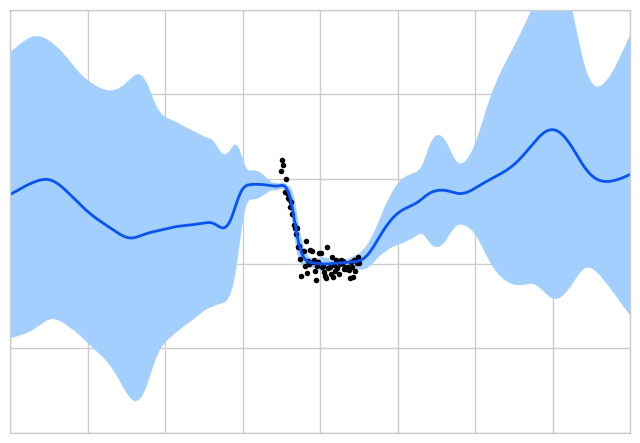
\includegraphics[width=.45\textwidth]{figs/bellBNN-mean-std}
    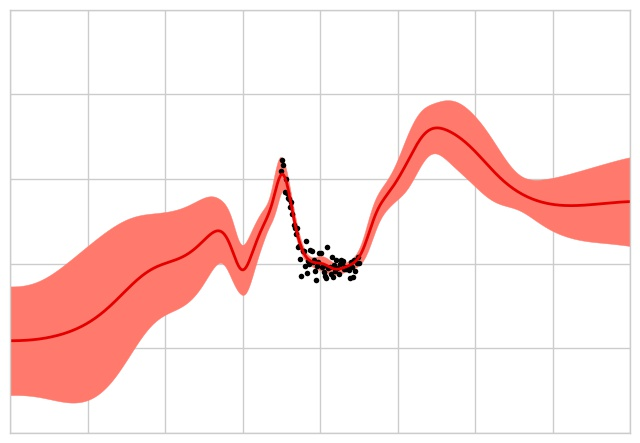
\includegraphics[width=.45\textwidth]{figs/red-bell-GPP-BNN-mean-std}
    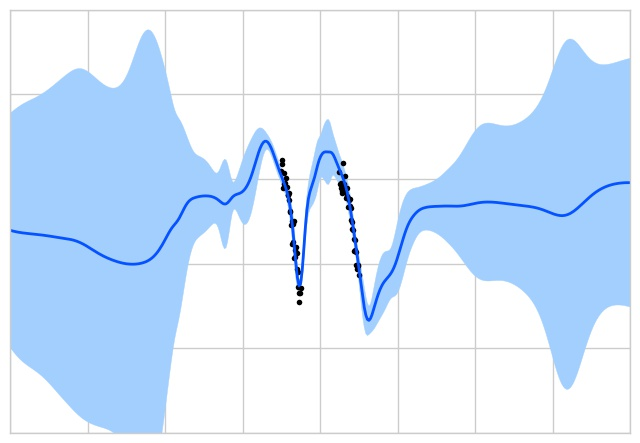
\includegraphics[width=.45\textwidth]{figs/cosBNN-mean-std}
    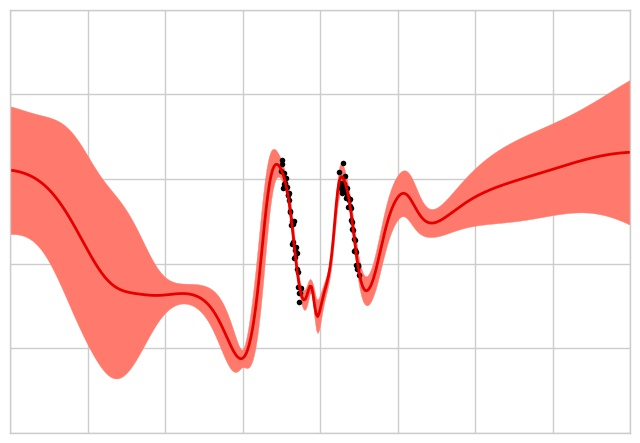
\includegraphics[width=.45\textwidth]{figs/red-cos-GPP-BNN-mean-std}
    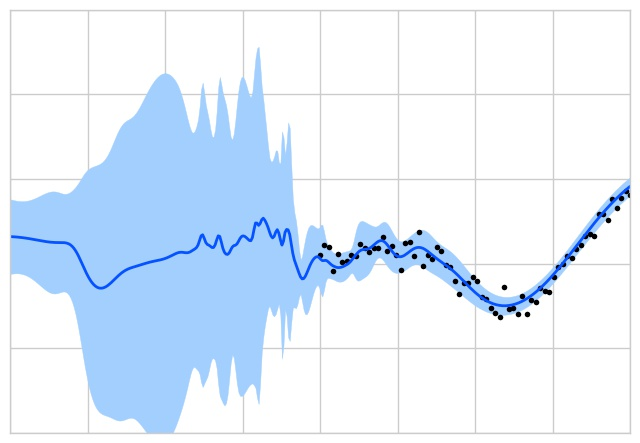
\includegraphics[width=.45\textwidth]{figs/cubeBNN-mean-std}
    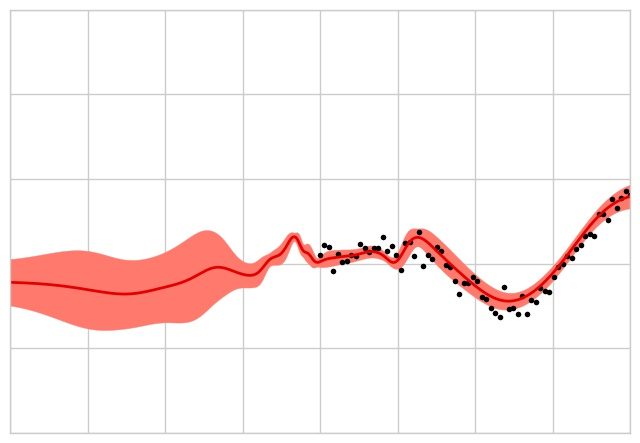
\includegraphics[width=.45\textwidth]{figs/red-cube-GPP-BNN-mean-std}
    \caption{The left column of plots are  Bayesian neural networks trained with a standard
             normal prior distribution on the weights. The right column are Bayesian 
             neural nets trained using the optimized prior found by doing step 1 in section 2.1. 
             The dots are samples from the data distribution. 
             The dark lines are the means of the posteriors and the 
             shaded regions are 95\% confidence intervals.}
    \label{fig:my_label}
\end{figure}

\subsection{Results}

In these toy cases, using smooth, infinitely differentiable functions to generate the datasets, the rbf kernel assumption proves to be a good one. Notice that the BNNs trained using the GP matched prior fit the data better and have more reasonable uncertainty envelopes.

\newpage

\subsubsection*{Acknowledgements}

The authors would like to thank Brian Ning and Guodong Zhang for helpful comments.

\section*{References}

Blundell, Charles, Cornebise, Julien, Kavukcuoglu, Koray, and Wierstra, Daan. Weight uncertainty
in neural networks.{\it  arXiv preprint arXiv:1505.05424, 2015. }


Danilo J Rezende, Shakir Mohamed, and Daan Wierstra. Stochastic backpropagation and approximate
inference in deep generative models. In { \it Proceedings of the 31st International Conference on
Machine Learning} (ICML-14), pages 1278–1286, 2014.

Diederik P Kingma and Max Welling. Auto-encoding variational bayes. arXiv preprint
arXiv:1312.6114, 2013.

Diederik Kingma and Jimmy Ba. Adam: A method for stochastic optimization.{\it arXiv preprint
arXiv:1412.6980, 2014}

Dougal Maclaurin, David Duvenaud, Matthew Johnson, and Ryan P. Adams. Autograd: Reversemode
differentiation of native Python, 2015.

Soumya Ghosh, Finale Doshi-Velez Model Selection in Bayesian Neural Networks via Horseshoe Priors
{\it arXiv preprint arXiv:1705.10388, 2016  }

\end{document}